% ----------------------------------------------------------
\chapter{Diagramas UML}
\label{cha:testesgraficos}
\index{Diagramas UML}
% ----------------------------------------------------------

Este apêndice reúne os diagramas \gls{UML} elaborados, com o auxílio da
ferramenta PlantUML, ao longo da modernização do sistema, desde a base
algorítmica em Java (\textit{Desktop}) até a reescrita final em
Python/Streamlit. Os diagramas de classes, de atividades e de sequência de cada
versão complementam a descrição apresentada no corpo do texto. Cada diagrama
aparece em uma figura individual, com seção e legenda próprias, o que permite
a referência cruzada nas demais seções do trabalho.

\section{Diagrama de Classes --- Java}
\label{sec:diagclassejava}

\begin{figure}[htbp]
	\caption{Diagrama de classes.}
	\centering
		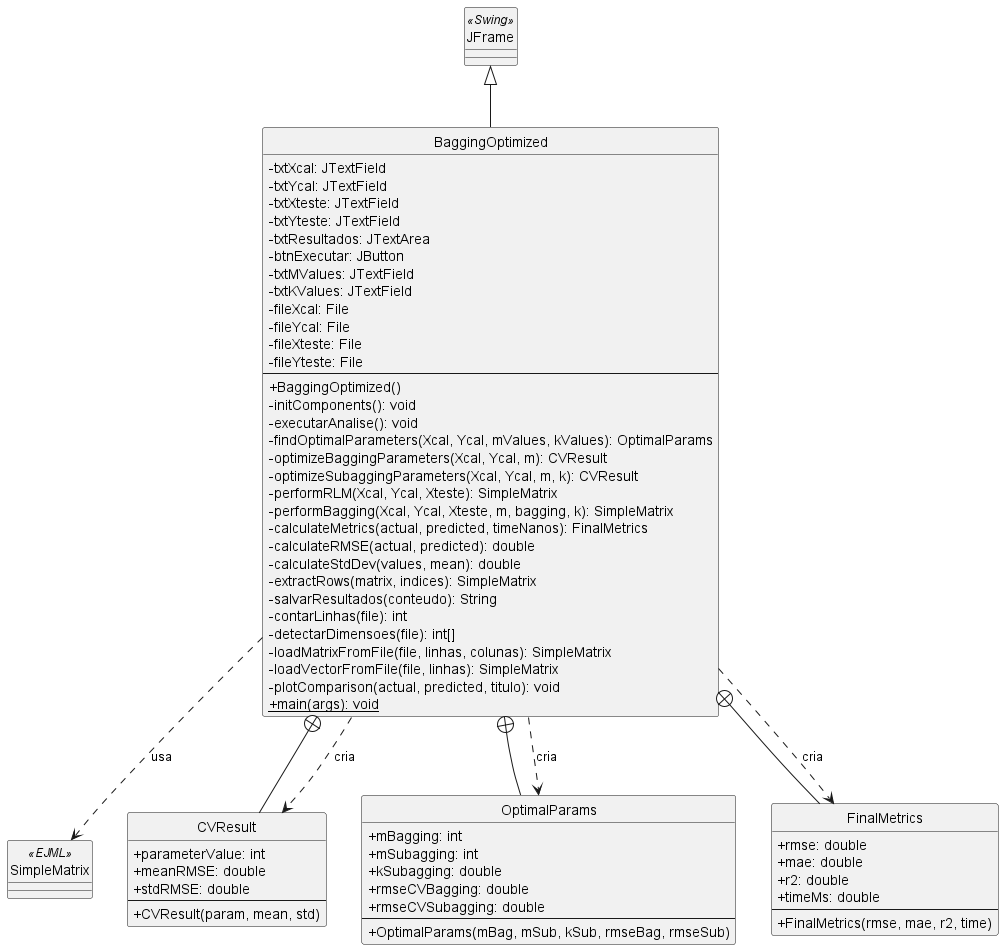
\includegraphics[width=1.00\textwidth]{./outros/fig/E_Diagramas/out/diag_classe/BaggingOptimized_Classe.png}
	\caption*{Fonte: \oautor}
	\label{fig:BaggingOptimized_Classe}
\end{figure}

\newpage
\section{Diagrama de Atividade --- Java}
\label{sec:diagatividadejava}

\begin{figure}[htbp]
	\caption{Diagrama de atividades.}
	\centering
		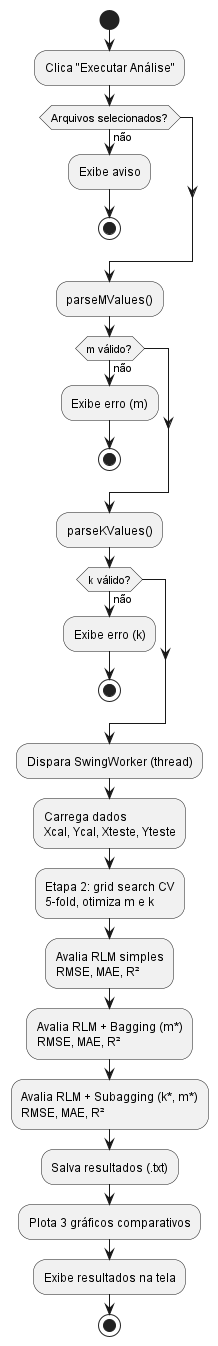
\includegraphics[width=0.20\textwidth]{./outros/fig/E_Diagramas/out/diag_sequencia/BaggingOptimized_Atividade.png}
	\caption*{Fonte: \oautor}
	\label{fig:BaggingOptimized_atividades}
\end{figure}

\newpage
\section{Diagrama de Sequência --- Java}
\label{sec:diagsequenciajava}

\begin{figure}[htbp]
	\caption{Diagrama de sequência.}
	\centering
		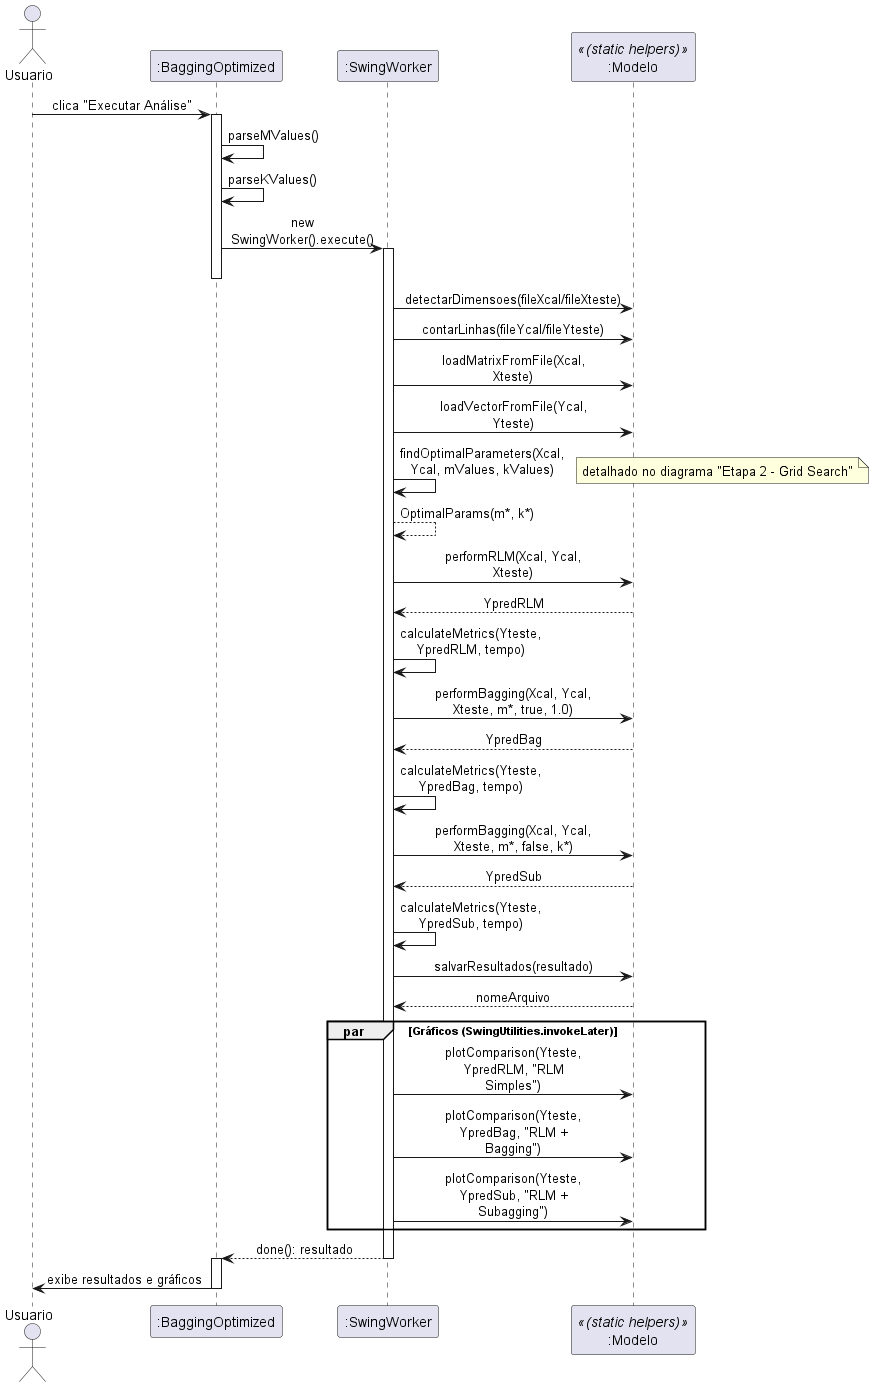
\includegraphics[width=0.75\textwidth]{./outros/fig/E_Diagramas/out/diagrama/BaggingOptimized_FluxoCompleto.png}
	\caption*{Fonte: \oautor}
	\label{fig:BaggingOptimized_sequencias}
\end{figure}

\newpage
\section{Diagrama de Atividades --- Java (PlantUML)}
\label{sec:diagatividadejavaplantuml}

\begin{figure}[htbp]
	\caption{Diagrama de atividade Java PlantUML .}
	\centering
		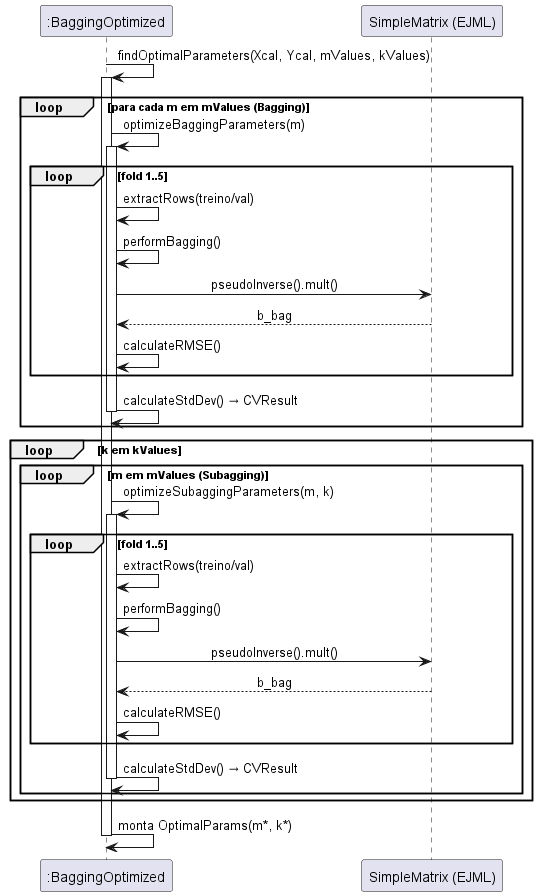
\includegraphics[width=0.50\textwidth]{./outros/fig/E_Diagramas/out/diagrama02/Etapa2_GridSearch_CV.png}
	\caption*{Fonte: \oautor}
	\label{fig:BaggingOptimized_atividade}
\end{figure}

\newpage
\section{Diagrama de Atividades --- Streamlit}
\label{sec:diagatividadestreamlit}

\begin{figure}[htbp]
	\caption{Diagrama de atividade Python PlantUML.}
	\centering
		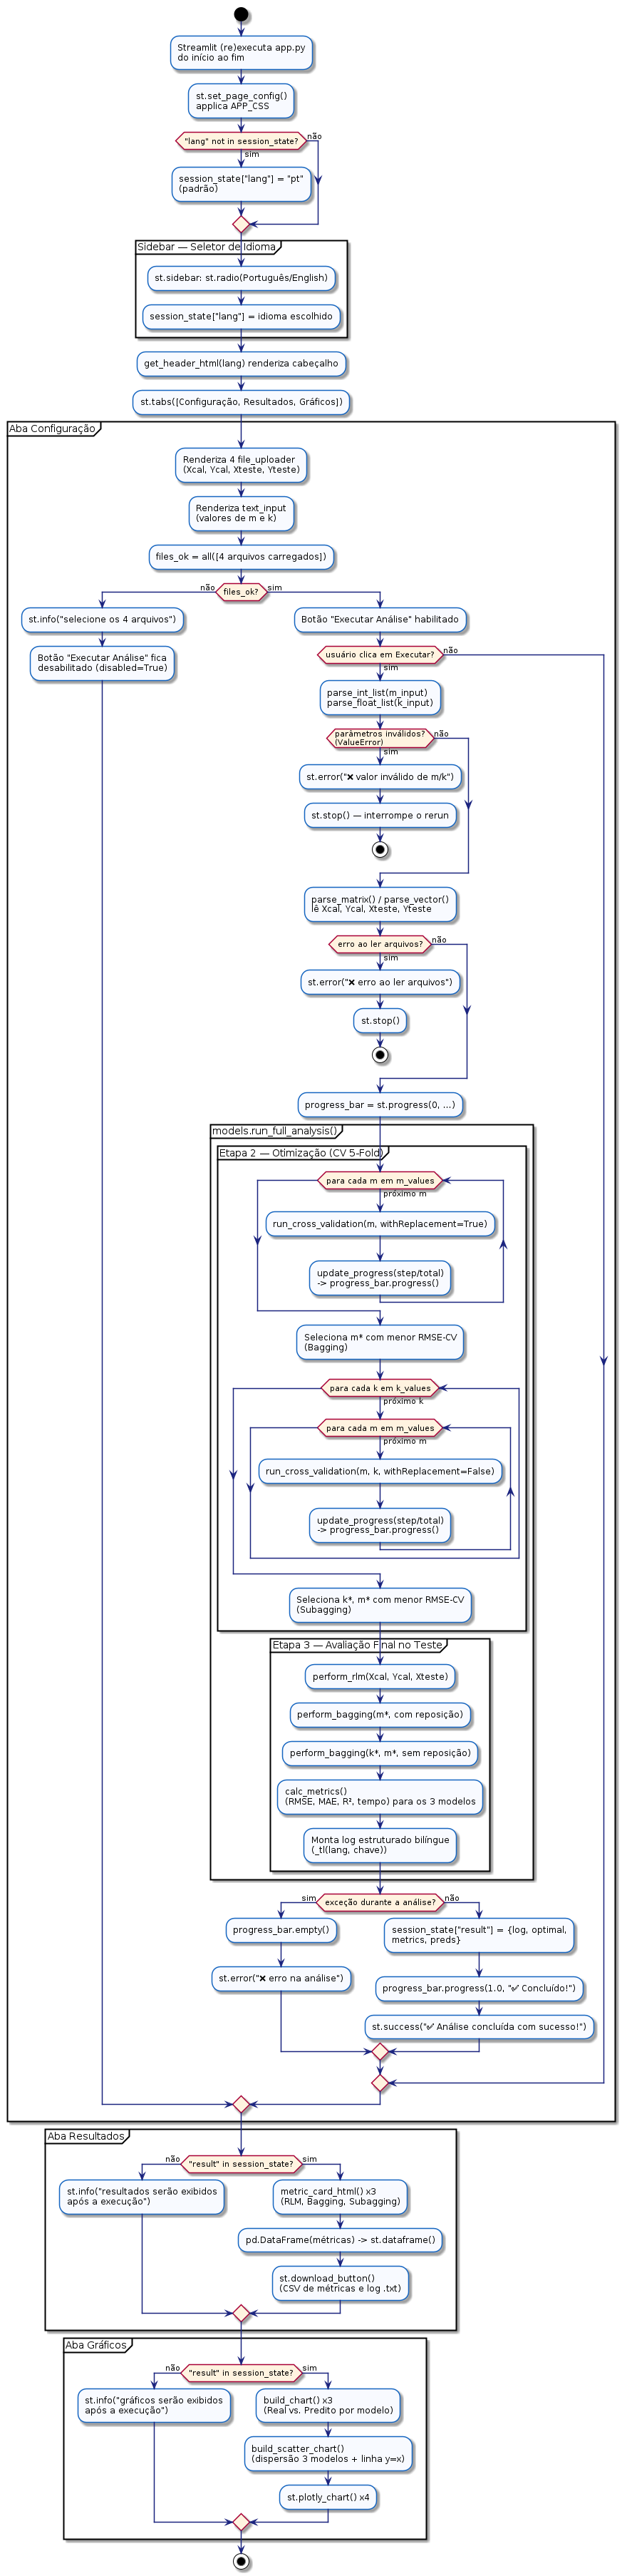
\includegraphics[width=0.30\textwidth]{./outros/fig/E_Diagramas/streamlit/diagrama_atividades_streamlit.png}
	\caption*{Fonte: \oautor}
	\label{fig:BaggingOptimized_atividade2}
\end{figure}

\newpage
\section{Diagrama de Classes (Módulos) --- Streamlit}
\label{sec:diagclassesstreamlit}

\begin{figure}[htbp]
	\caption{Diagrama de classes (módulos) PlantUML.}
	\centering
		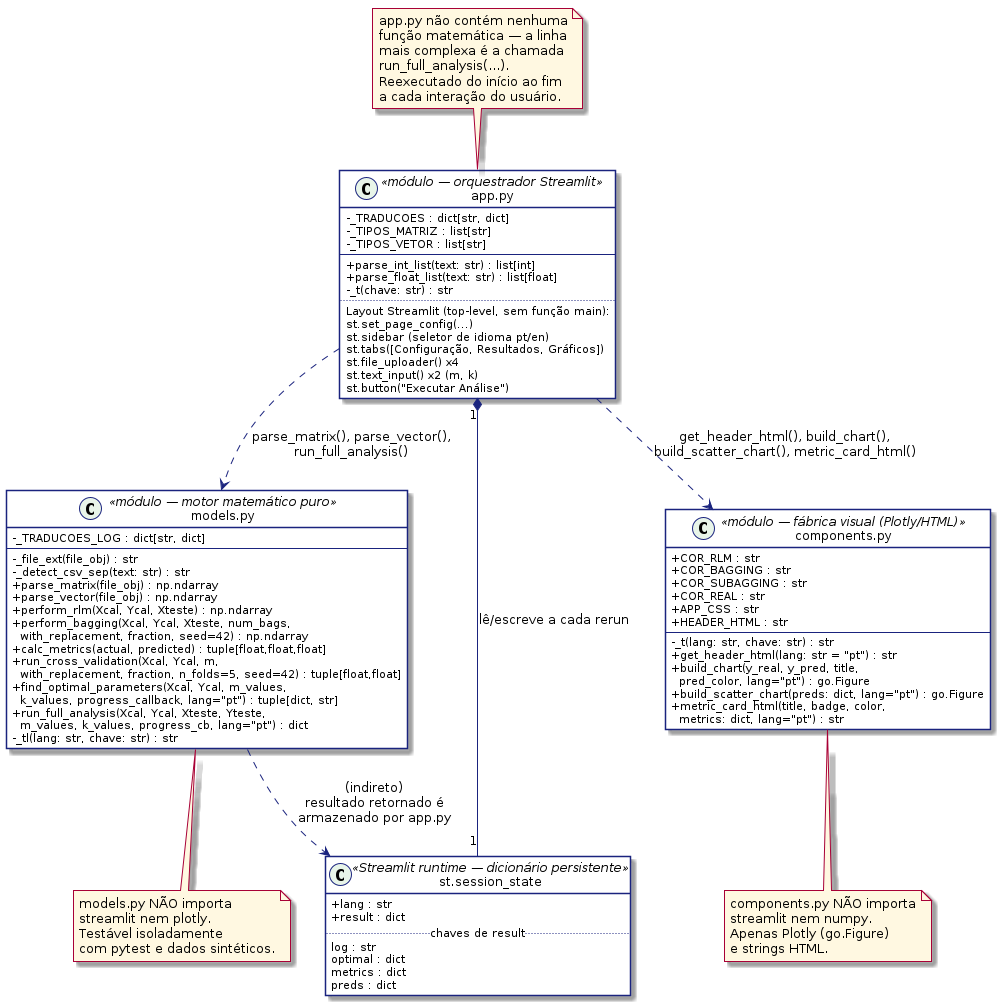
\includegraphics[width=0.85\textwidth]{./outros/fig/E_Diagramas/streamlit/diagrama_classes_streamlit.png}
	\caption*{Fonte: \oautor}
	\label{fig:BaggingOptimized_classe3}
\end{figure}

\newpage
\section{Diagrama de Sequência --- Streamlit}
\label{sec:diagsequenciastreamlit}

\begin{figure}[htbp]
	\caption{Diagrama de sequência PlantUML.}
	\centering
		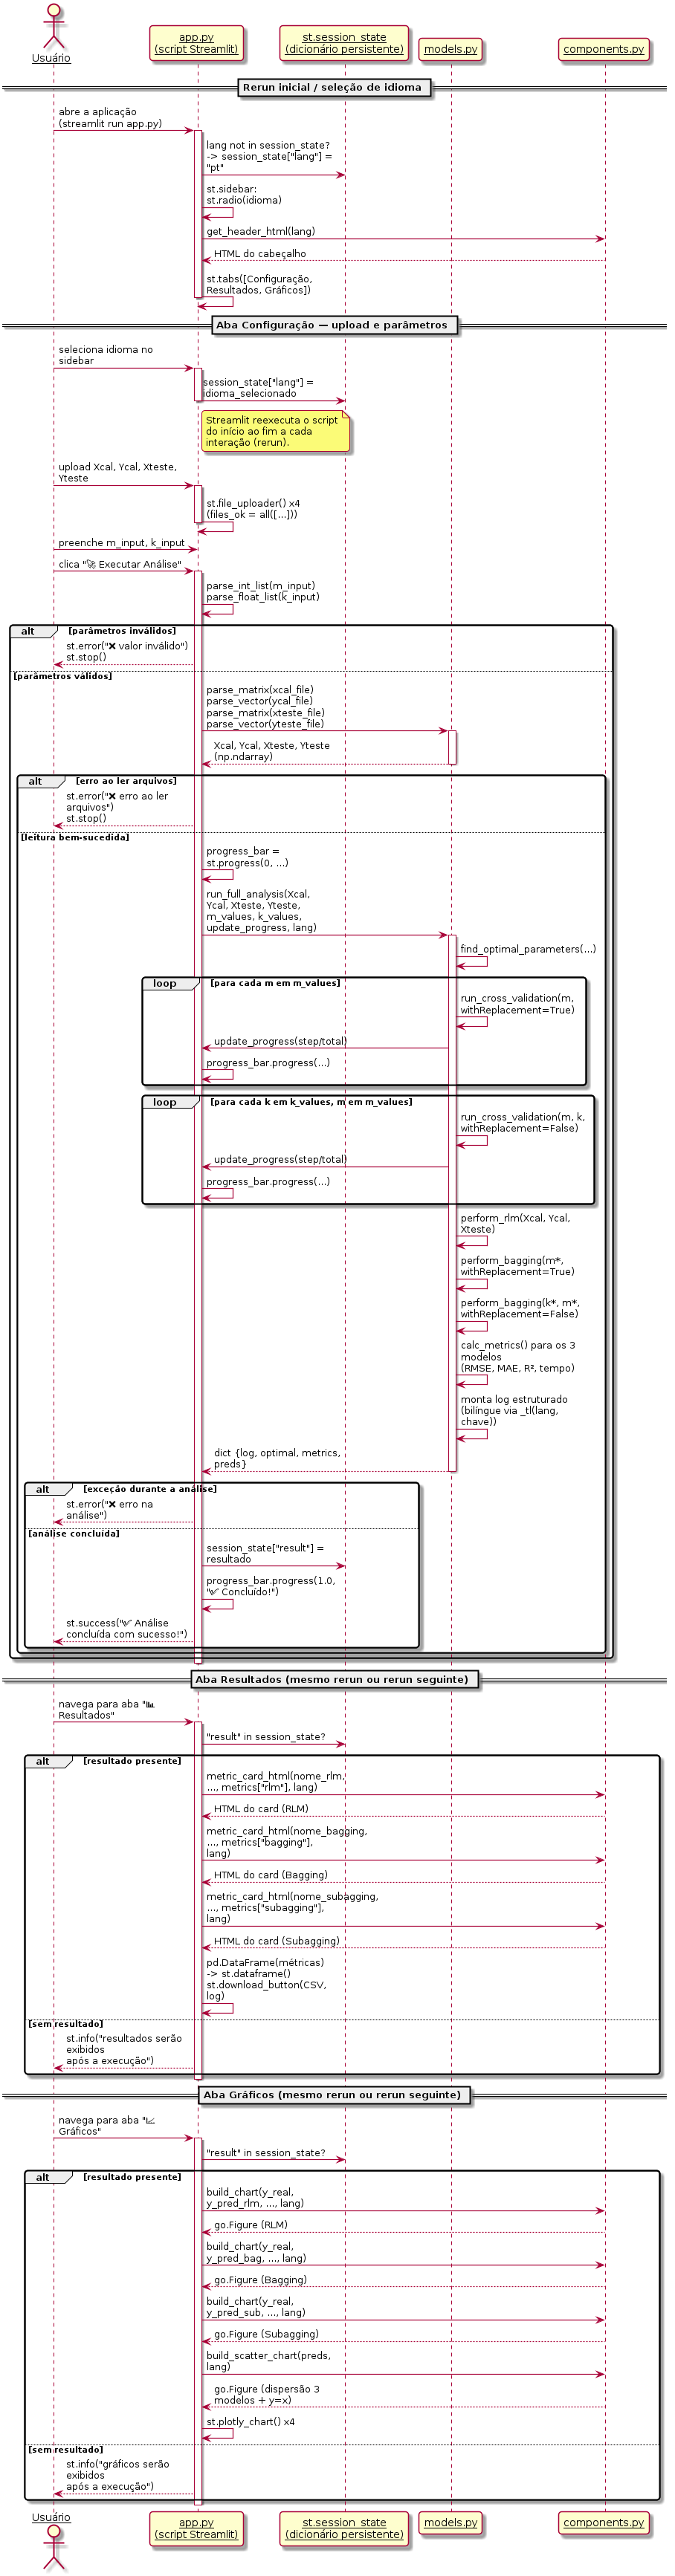
\includegraphics[width=0.30\textwidth]{./outros/fig/E_Diagramas/streamlit/diagrama_sequencia_streamlit.png}
	\caption*{Fonte: \oautor}
	\label{fig:BaggingOptimized_sequencia2}
\end{figure}

